\documentclass{beamer}

\usetheme{Copenhagen}
\usecolortheme{default}

\usepackage{dot2texi}
\usepackage{tikz}
\usetikzlibrary{shapes,arrows}
\usepackage{bookmark}
\usepackage{graphicx}
\usepackage{todonotes}
\usepackage{hyperref}


\def\email#1{{\tt#1}}

\mode<handout>{%
  \usepackage{pgfpages}
  \pgfpagesuselayout{resize to}[a4paper]
}

\title{Applicability of SSM and UML for Designing a Search Application for the British Broadcasting Corporation (BBC)}
\author{Ross Fenning\inst{1}
  \and Huseyin Dogan\inst{2}
  \and Keith Phalp\inst{2}}
\institute{BBC, UK \\ \email{Ross.Fenning@bbc.co.uk}
  \and Bournemouth University, UK \\ \email{\{hdogan,kphalp\}@bournemouth.ac.uk}}
\date{2014-11-05}

%gets rid of bottom navigation bars
\setbeamertemplate{footline}[frame number]{}

%gets rid of navigation symbols
\setbeamertemplate{navigation symbols}{}

\begin{document}

\begin{frame}[plain]
  \titlepage
\end{frame}

% Background
\begin{frame}
  \frametitle{About Me}
  \begin{itemize}
    \item Senior Software Engineer
    \item Future Media: Content Discovery: Search
  \end{itemize}
\end{frame}

\begin{frame}
  \frametitle{What is BBC Search?}
  \framesubtitle{i.e. What do I work on?}
  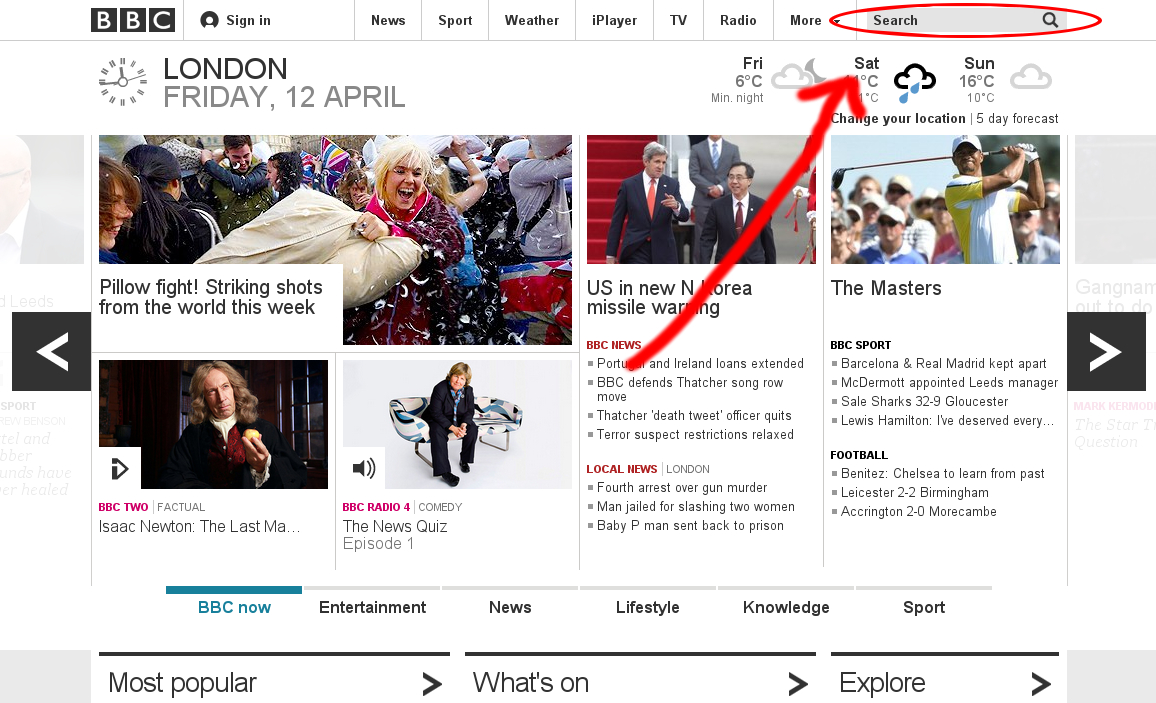
\includegraphics[width=\linewidth]{homepage.png}
\end{frame}

% Design Goals
\begin{frame}
  \frametitle{Design Goals}
  \framesubtitle{Motivation}
  \begin{itemize}
    \item Showcase
    \item Fresh approach
    \item Inform improvements?
    \item Contextualisation via SSM
    \item Bring audience closer to the design
  \end{itemize}
\end{frame}

\begin{frame}
  \frametitle{Design Goals}
  \framesubtitle{Requirements}
  \begin{itemize}
    \item Existing search application serves a wide variety of use cases
    \item The Search application should integrate where possible with other existing systems
    \item Website is very high traffic
    \item Different parts of the overall website are maintained by distinct teams
    \item Varying applications, data stores and content management systems
  \end{itemize}
\end{frame}

\begin{frame}
  \frametitle{What is SSM?}
  \framesubtitle{Peter Checkland}
  \begin{center}
    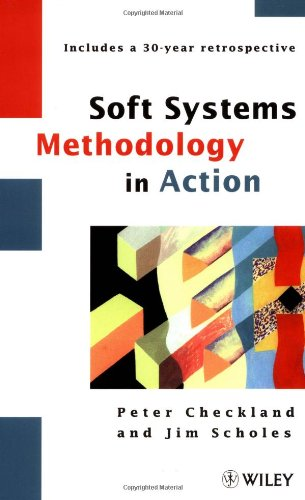
\includegraphics[height=0.8\textheight]{ssma.jpg}
    \quad
    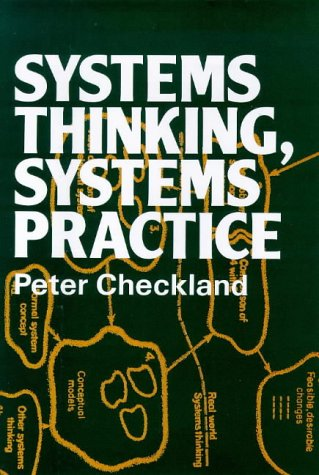
\includegraphics[height=0.8\textheight]{stsp.jpg}
  \end{center}
\end{frame}

\begin{frame}
  \frametitle{Problem Contextualisation through SSM}
  \begin{itemize}
    \item Claim: ``Hard systems'' (e.g. UML) take an ontological view:
    \begin{itemize}
      \item What components are there?
      \item Who are the actors?
      \item What are the interactions between actors and components?
      \item What are the computations or workflows steps/stages?
    \end{itemize}
    \pause \item Claim: SSM takes an epistemological view:
    \begin{itemize}
      \item How does the holistic search system transform user needs to content and information?
      \item How can the purposeful activity be monitored?
      \item How is the activity observed by different observers?
      \item How can different observers inform the activity?
    \end{itemize}
    \pause \item Dogan and Henshaw (2010) showed a transition from soft systems to hard models
  \end{itemize}
\end{frame}

\begin{frame} 
  \frametitle{Problem Contextualisation through SSM}
  \framesubtitle{Rich Picture}
  \pause 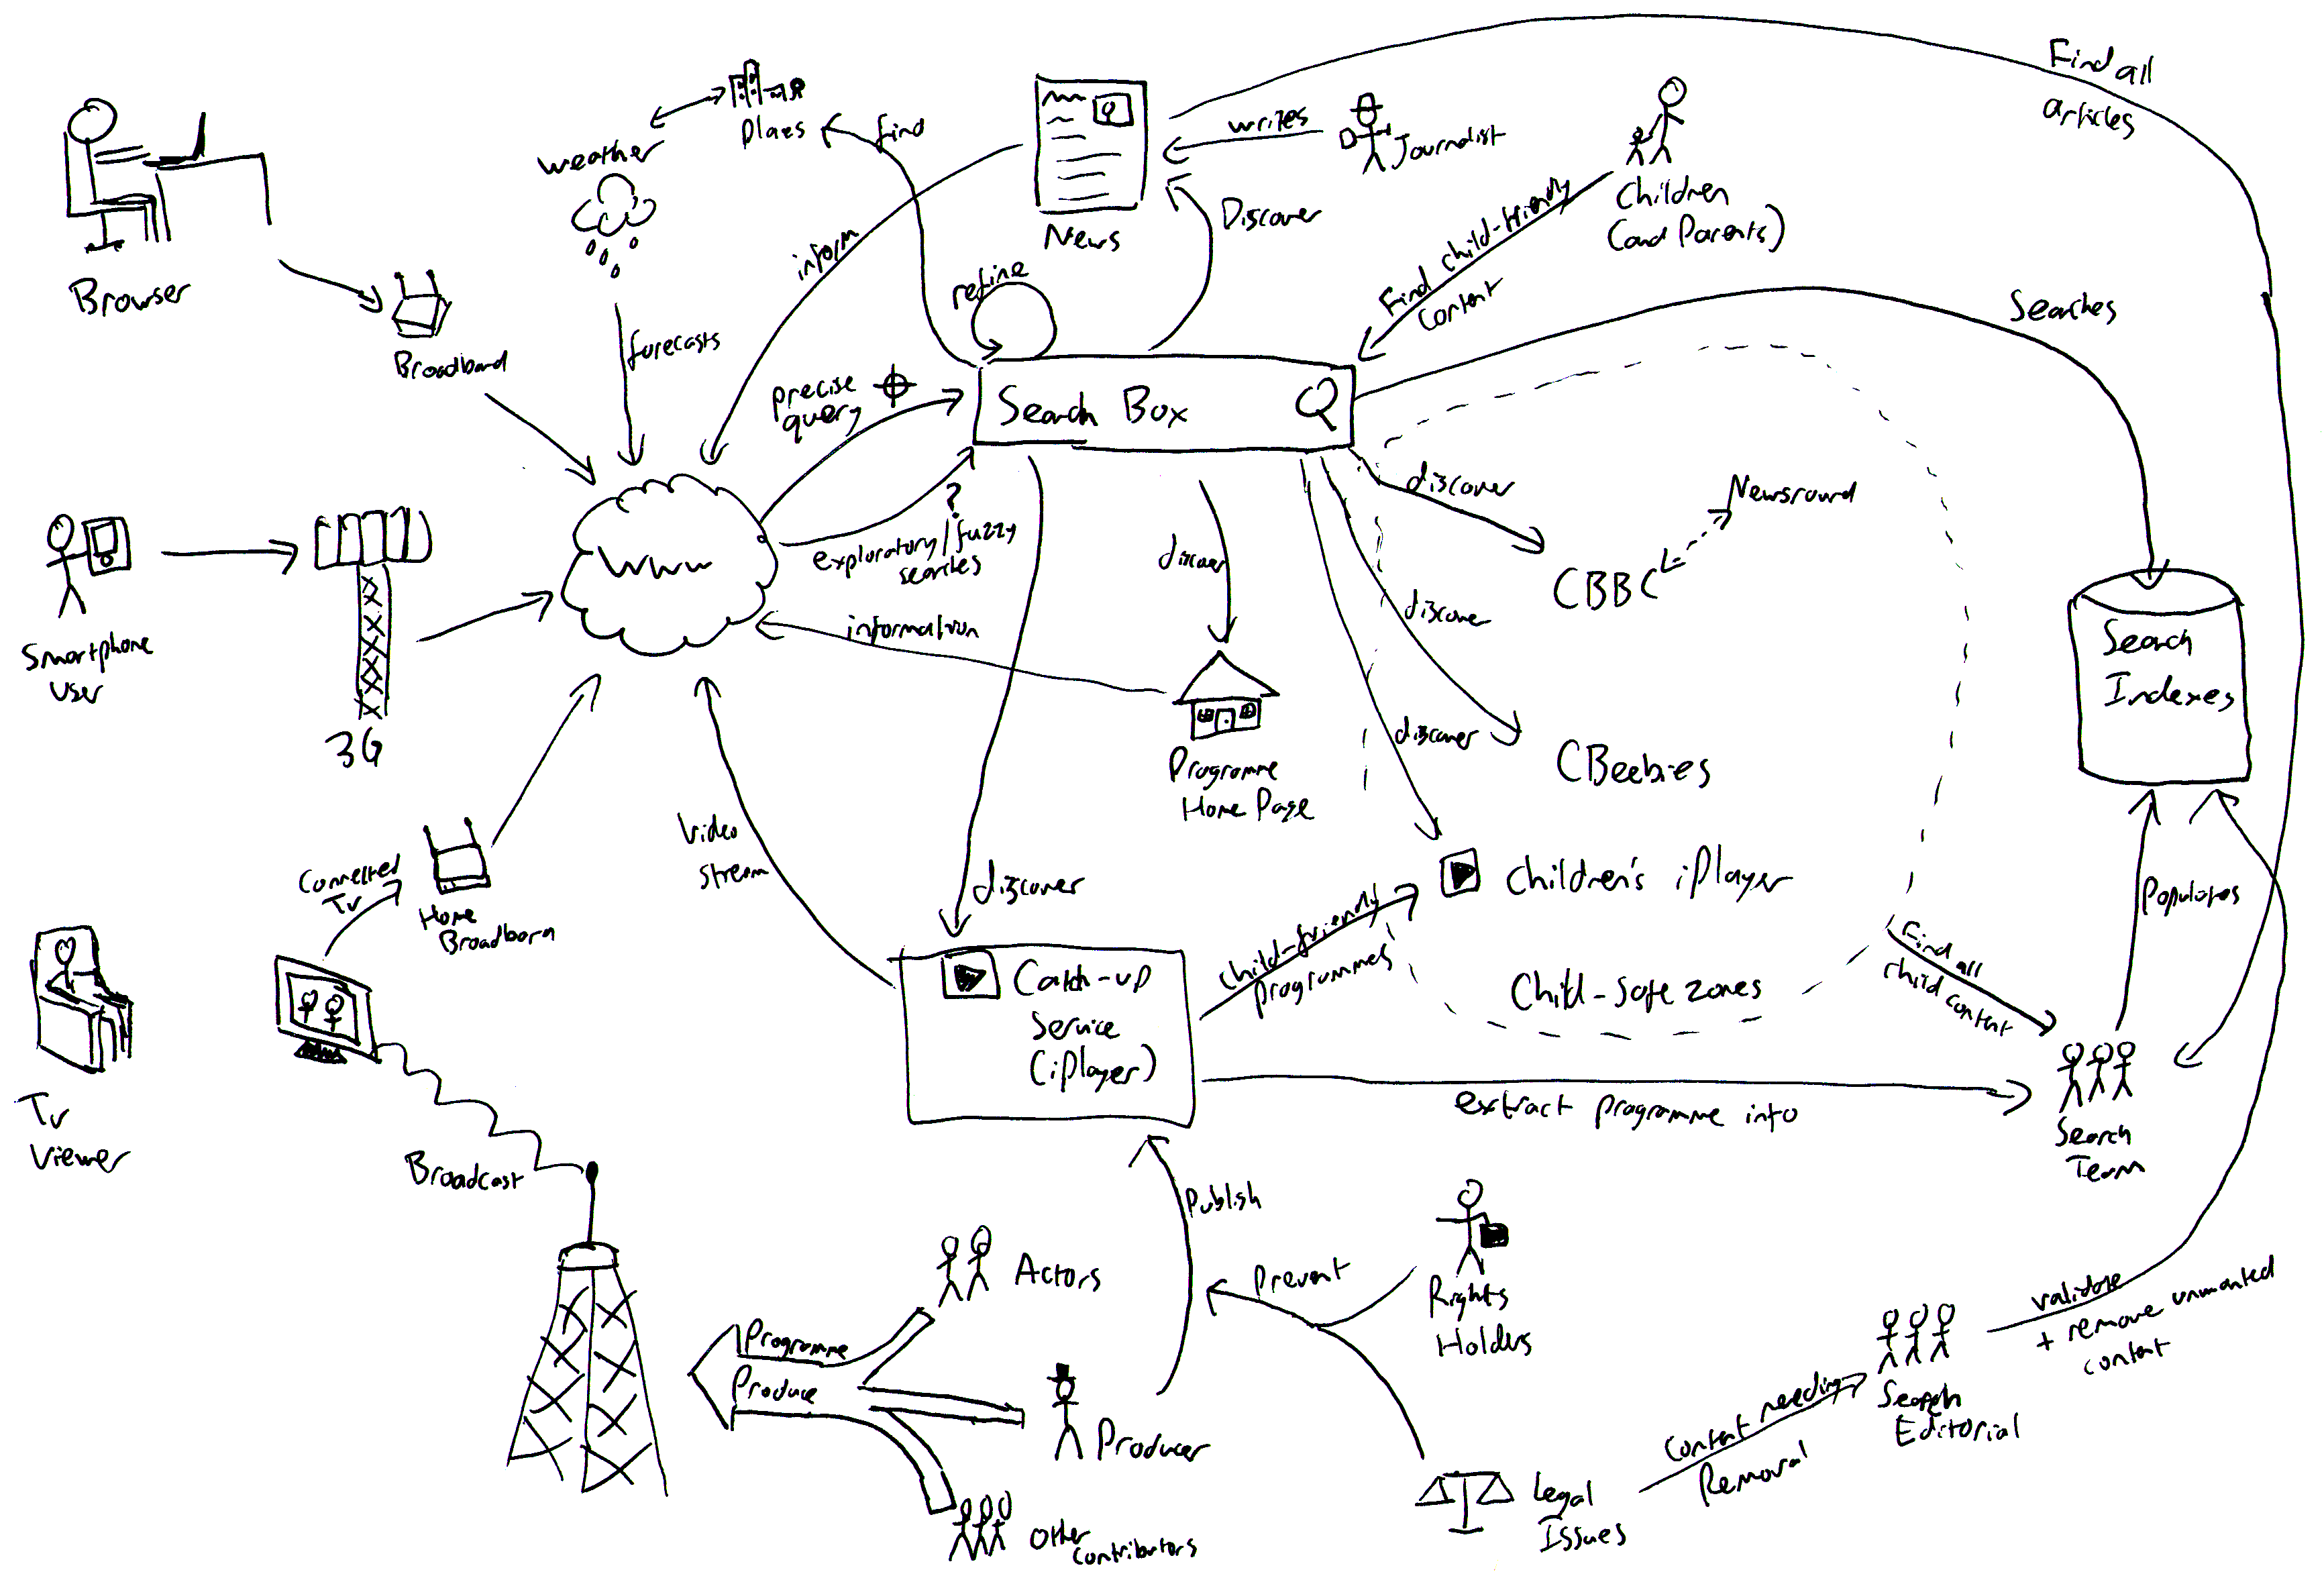
\includegraphics[width=\linewidth]{rich-picture.png}
\end{frame}

% Extracting use cases
\begin{frame}[fragile]
  \frametitle{Use Case Extraction}
  \framesubtitle{Identifying users}
  \begin{center}
    \begin{dot2tex}[dot,scale=0.6]
      digraph G {
        rankdir=LR;
        node;
        "Rich Picture" -> Users
        Users -> "Direct Users";
        Users -> "Indirect Users";
      }
    \end{dot2tex}
    \quad
    \begin{itemize}
    \item Identify all users
    \item \emph{Direct} vs. \emph{meta-level} users
    \item Direct use cases should emerge from the rich picture
    \item Note that separation is \emph{subjective}
    \item Use cases can change if rich picture changes
    \end{itemize}
  \end{center}
\end{frame}

% Designing behaviour for indirect users
\begin{frame}
  \frametitle{Use Case Extraction}
  \framesubtitle{Meta-level Users}
  \begin{itemize}
  \item Meta-level users do not transition to the use case models directly
  \item We should still consider how meta-level users are affected by emergent properties of the holistic system
    \begin{itemize}
    \item Actors
    \item Journalists
    \item Parents
    \item Other Future Media products?
    \item Future Media staff
    \end{itemize}
  \end{itemize}
\end{frame}

% Designing behaviour for direct users
\begin{frame}
  \frametitle{Use Case Extraction}
  \framesubtitle{Direct Users}
  \begin{itemize}
    \item Direct users transition directly to actors into a UML use case diagram
    \item Use cases should derive from and be justifiable by the rich picture
    \item Direct users divide up into \emph{content production} and \emph{audience}
    \item Examples of each:
    \begin{itemize}
      \item News editors
      \item Users of the search web application
    \end{itemize}
  \end{itemize}
\end{frame}

\begin{frame}
  \frametitle{Use Case Extraction}
  \framesubtitle{UML Use Case Diagram}
  \includegraphics[width=\linewidth]{use_case.png}
\end{frame}

\begin{frame}
  \frametitle{System Behaviour}
  \framesubtitle{Programmes metadata producer}
  \includegraphics[width=\linewidth]{plant_sequence_producer.png}
\end{frame}

\begin{frame}
  \frametitle{System Behaviour}
  \framesubtitle{Website user}
  \begin{center}
    \includegraphics[height=0.8\textheight]{plant_sequence_user.png}
  \end{center}
\end{frame}

\begin{frame}
  \frametitle{System Behaviour}
  \framesubtitle{Lazy-loading page via AJAX}
  \begin{center}
    \includegraphics[height=0.8\textheight]{plant_sequence_ajax.png}
  \end{center}
\end{frame}

% Domain modelling for search -- model business rules as per benefits shown in background, but also keep it generic
\begin{frame}
  \frametitle{Domain Modelling}
  \begin{itemize}
    \item Use cases identify types of content users want to search
    \item Things we want to model should emerge from the rich picture
    \item ``TV'' and ``Radio''? Or just ``programmes''?
    \item Ontology designs exist for specific content domains, e.g. programmes, sport
    \item A search across all content types needs a model to span all domains
  \end{itemize}
\end{frame}

\begin{frame}
  \frametitle{Domain Modelling}
  \framesubtitle{Maximal Class Diagram/Domain Model}
  \begin{center}
    \pause \includegraphics[height=0.8\textheight]{plant_model.png}
  \end{center}
\end{frame}

% Discussion and Analysis -- Use cases - More SSM needed?

\begin{frame}
  \frametitle{Discussion}
  \framesubtitle{Use Cases}
  \begin{itemize}
    \item Use case model seems justifiable at a high level
    \item Many use cases and variations are missing
    \item More collaborative and continuous use of SSM should incorporate respective domain experts
    \item More user testing, audience feedback, requirements-gathering, etc. needed
    \item Possible need to iterate SSM processes towards a collection of use case models
  \end{itemize}
\end{frame}

\begin{frame}
  \frametitle{Discussion}
  \framesubtitle{System Behaviour}
  \begin{columns}[T]
    
    \column{0.5\textwidth}
    
    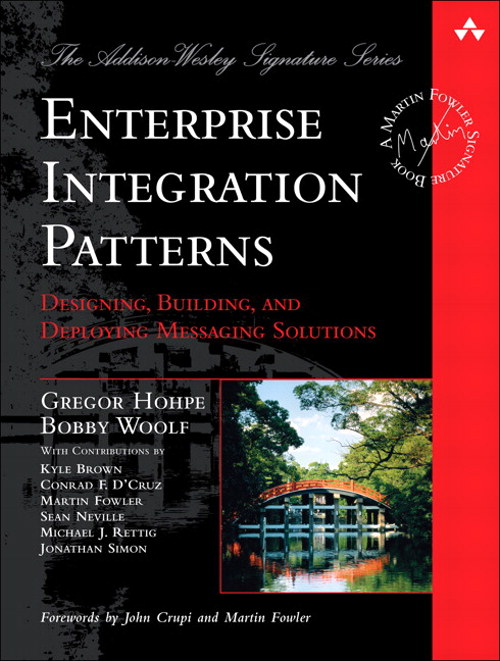
\includegraphics[width=\linewidth]{eip.jpg}
    
    \column{0.5\textwidth}
    
      \begin{itemize}
      \item Asynchronous messaging
      \item Claim Check
      \item Content Enricher
      \item Index vs. warehouse?
      \item Objective evaluation?
      \end{itemize}

  \end{columns}
\end{frame}

% Discussion and Analysis -- Domain Model -- Polymorphism
\begin{frame}
  \frametitle{Discussion}
  \framesubtitle{Domain Model}
  \begin{itemize}
    \item Large, maximal data model useful as communication artefact
    \item Aggregate models hard to keep in sync with changes in respective domains
    \item Does Search need to model all of this?
      \begin{itemize}
        \item Polymorphic supertype -- ``Thing'' class?
        \item Facade -- ``SearchResult'' class?
      \end{itemize}
  \end{itemize}
\end{frame}

% Discussion and Analysis -- Domain Model -- Duck Typing
\begin{frame}
  \frametitle{Discussion}
  \framesubtitle{Schemalessness and Duck Typing}
  \begin{itemize}
    \item Statically typed approach: A \emph{Place} always has a ``today's weather forecast'' attribute
    \item Dynamically (``duck'') typed approach: any entity can have a ``today's weather forecast'' attribute and we display this forecast if that attribute is present
    \item Allows other entities in future to have forecasts too (e.g. \emph{Events} such as football matches)
    \item Search application can store all fields from upstream sources and choose when to start using them
  \end{itemize}
\end{frame}

% Discussion -- More SSM: 3 Es?
\begin{frame}
  \frametitle{Discussion}
  \framesubtitle{Overall Model: Use cases, behaviour and domain}
  \begin{itemize}
    \item Looks good
    \item Agile? MVP? Test assumptions?
    \item How do we monitor for ``3 Es''?
      \pause \begin{itemize}
        \item Efficacy -- Does the system do what we intended?
        \item Efficiency -- Does it minimise use of resources?
        \item Effectiveness -- Does it fit into our long term goals?
      \end{itemize}
  \end{itemize}
\end{frame}

% Shortcomings -- Agile?
\begin{frame}
  \frametitle{Evaluation and Difficulties}
  \framesubtitle{Detailed Design and Agile}
  \begin{itemize}
    \item High-level design lacks detail (not surprisingly)
    \item Agile encourages delivering something tangible early
    \item Shouldn't the full detailed design emerge iteratively?
    \item Can we iteratively build up and maintain hard models?
    \item Can we defer pending questions in our hard models until we know more?
    \item SSM encourages continuous feedback cycles -- does this align with Agile?
    \item Bustard, Dave, and Frank Keenan. ``Soft Systems Methodology: An Aid to Agile Development?.''
      In \emph{Information Systems Development}, pp. 25-38. Springer US, 2009.
  \end{itemize}
\end{frame}

% Shortcomings -- Performance? NFRs?
\begin{frame}
  \frametitle{Evaluation and Difficulties}
  \framesubtitle{Non-functional Requirements}
  \begin{itemize}
    \item Performance
    \item Availability/uptime
    \item Latency between publishing and searchability
    \item Secure/robust
    \item Maintainability -- the holistic system includes developers!
  \end{itemize}
\end{frame}

\begin{frame}
  \frametitle{Further Work}
  \begin{itemize}
    \item Can SSM take a more formal place in our processes?
    \item Are there more parallels between Agile and SSM that engineers in industry have yet to appreciate?
    \item Can we streamline modelling and design to fit an iterative process?
  \end{itemize}
\end{frame}

\begin{frame}
  \frametitle{Questions}
  \begin{center}
    \url{http://rossfenning.co.uk/pages/papers.html}\\
    \texttt{Ross.Fenning@bbc.co.uk}\\
    \texttt{@Avenger\_Penguin}
  \end{center}
\end{frame}

\end{document}
